\documentclass[12pt]{report}
\usepackage[utf8]{inputenc}

\usepackage{geometry}
\usepackage[spanish]{babel}
\renewcommand{\baselinestretch}{1.5}
\geometry{letterpaper, margin=2.5cm}
\usepackage{graphicx}
\usepackage{hyperref}
\urlstyle{same}
\usepackage{fancyhdr}
\usepackage{amsmath}
\usepackage{braket,mleftright}
\mleftright
 
\usepackage[sorting=none]{biblatex}
 
\addbibresource{references.bib}

\begin{document}

\begin{titlepage}
   \begin{center}
       \vspace*{1cm}
       
       
       \large
       \textbf{Estimación del espectro energético de la radiación producida por la interacción de cascadas atmosféricas extensas con la corteza terrestre}
       
       %\large
       %\vspace{0.5cm}
        %¿Subtítulo?
 
       \vspace{1.5cm}
 
       \small
       Propuesta de tesis de pregrado para optar al título de \\
       Físico
       
       
       \normalsize
       \textbf{Ricardo de León Barrios}
       
       \small
       \vspace{1cm}
       Director\\
       \textbf{Mauricio Suárez Durán}$^1$\\
       Doctor en Ciencias Naturales (Física)
       
       \vspace{1cm}
       Codirector\\
       \textbf{Luis A. Núñez de Villavicencio}$^1$\\
       Doctor en Física\\
       
       \vspace{1cm}
       $^1$\textit{Grupo de Investigación en Relatividad y Gravitación, UIS}
 
       \vfill
       
       
 
       %\vspace{0.8cm}
 
       
 
       \small
       Escuela de Física\\
       Facultad de Ciencias\\
       Universidad Industrial de Santander\\
       Bucaramanga, Colombia\\
       2020\\
       \vspace{0.3cm}
       
\includegraphics[width=0.25\textwidth]{logo/logoUIS.png}
 
   \end{center}
\end{titlepage}

%---------------------------------------

\section*{Resumen}


%------------------------------------
\section*{Introducción}








%--------------------------
\section*{Marco teórico}

\subsection*{Sobre rayos cósmicos y cascadas atmosféricas extensas}

\normalsize

Los rayos cósmicos son partículas cargadas y altamente energéticas provenientes del espacio. Se pueden clasificar entre aquellas provenientes de nuestro propio Sol y de fuentes externas al sistema solar, ya sea dentro de la Vía Láctea, o de fuentes extragalácticas. \cite{moldwin2008introduction} A pesar de que se les denomina \textit{rayos}, comúnmente se excluye de esta definición a la radiación electromagnética \cite{NASACosmicopia}, limitándose exclusivamente a partículas con masa. La mayoría de los rayos cósmicos están compuestos por núcleos de elementos que van desde el más ligero, el hidrógeno, hasta núcleos de elementos pesados, como el hierro. También se incluyen otras partículas como electrones, neutrones, neutrinos, positrones y antiprotones. \cite{NASAImagine}

Las partículas de rayos cósmicos pueden llegar a alcanzar energías muy altas, de alrededor de 100 MeV, y velocidades de más del 99\% de la velocidad de la luz. \cite{moldwin2008introduction} Estas partículas formadas en eventos astrofísicos como llamaradas solares y supernovas se denominan \textbf{partículas primarias}. Cuando llegan a la atmósfera terrestre, interactúan con moléculas de aire (principalmente nitrógeno, oxígeno y argón, que son los mayores componentes de la atmósfera) y decaen en \textbf{partículas secundarias}, creando eventos llamados \textit{cascadas atmosféricas extensas}, o \textit{EAS}\footnote{Siglas en inglés, \textit{Extensive Air Showers}.}. Estas partículas secundarias tienen menos energía que las primarias que las crearon. Algunas partículas secundarias que se pueden formar en estas cascadas son piones y kaones, que a su vez, pueden decaer en muones y neutrinos. \cite{grieder2010extensive} También se pueden formar cascadas electromagnéticas (fotones), partículas alfa, protones, electrones y neutrones.

Para el estudio de los rayos cósmicos es importante la noción de flujo, que se define como el número de partículas que atraviesan una superficie por unidad de área, por unidad de tiempo. En el caso del flujo de rayos cósmicos en la parte superior de la atmósfera, existen varios factores que lo pueden afectar, tales como la actividad solar y el campo magnético terrestre. \cite{PhysRevD.98.030001}

De particular interés en la actualidad es el estudio del flujo de muones, con importantes aplicaciones para escaneos por radiografía y tomografía, de los cuales se hablará más a fondo en la siguiente sección. Los muones generalmente se forman por el decaimiento de piones, quienes a su vez se crean a partir del choque de núcleos atómicos de rayos cósmicos con partículas de la atmósfera. Los muones son bastante inestables, decayendo rápidamente por interacción débil. El tiempo de vida de los muones, medido en un marco de referencia inicial en reposo respecto a ellos, solo permitiría una distancia de viaje de menos de 500 metros para la mitad de estos (viajando al 99,97\% de la velocidad de la luz) antes de decaer en otras partículas; esto es sin tener en cuenta los efectos relativistas. Sin embargo, debido a las altas velocidades que alcanzan los muones, se deben tener en cuenta los efectos de la contracción de longitudes y la dilatación del tiempo. En este caso, desde nuestra perspectiva en la Tierra, la semivida de los muones se extiende debido a la dilatación temporal, siendo lo suficientemente larga como para detectarlos en la superficie de la Tierra, e incluso a varios cientos de metros bajo tierra, debido a su alto poder penetrativo. Desde la perspectiva de un marco de referencia inercial en reposo respecto de los muones, actúa la contracción espacial, haciendo que la distancia de viaje hacia la superficie de la Tierra sea más corta. \cite{cunningham2019high}

Dos principales métodos de detección de rayos cósmicos existen: uno de detección directa de las partículas primarias en la parte superior de la atmósfera, mediante el uso de globos de grandes altitudes y satélites, y un segundo método, que consiste en detectar, a nivel del suelo, las partículas secundarias y la radiación electromagnética creadas en las EAS. Estas formas de detección son denominadas detección \textit{directa} e \textit{indirecta}, respectivamente. El presente trabajo de investigación se asienta sobre el método de detección indirecta a nivel del suelo.

Una de las herramientas más importantes en la detección de partículas secundarias es el detector Cherenkov, cuyo funcionamiento se basa en el fenómeno de la radiación de Cherenkov: Así llamada por el físico soviético Pável Cherenkov, es la radiación electromagnética emitida cuando un medio dieléctrico es atravesado por una partícula cargada viajando a una velocidad superior a la de la luz en ese medio. \cite{jelley1955cerenkov} Este fenómeno se puede entender como un análogo electromagnético a la onda de choque que se crea cuando un objeto viaja a una velocidad que supera a la velocidad del sonido en un medio.

%---------------------------------------------------------


\subsection*{Sobre la corteza terrestre, y la radiografía y tomografía de muones}

La corteza es una delgada capa rocosa que cubre la superficie de la Tierra, siendo la capa más externa de la \textbf{geósfera} o tierra sólida. Se separa en dos tipos principales: oceánica y continental. La oceánica tiene un grosor promedio de 6 km, densidad promedio de 3 g cm$^{-3}$ y una edad de menos de 200 millones de años, mientras que la continental tiene un grosor promedio de 39 km, densidad promedio de 2,84 g cm$^{-3}$ y edad promedio de 1500 millones de años. \cite{mooney20101} La corteza terrestre \textit{flota} sobre el manto, teniendo este una densidad mayor. Puesto que la corteza oceánica tiene mayor densidad que la corteza continental, esta última \textit{flota más alto}, y los cuerpos masivos de agua se acumulan sobre la corteza oceánica. Esta condición de equilibrio entre corteza y manto se denomina isostasia. Los elementos más abundantes en la corteza son el oxígeno, el silicio y el aluminio, y los minerales más abundantes son los feldespatos, el cuarzo y los piroxenos. \cite{anderson2010geomorphology}

En este trabajo estudiaremos la interacción de las partículas de las EAS con la materia de la corteza terrestre, la cual modelaremos como la denominada \textit{roca estándar}. Esta es una representación del suelo bastante usada en la física de partículas y rayos cósmicos, y el estudio de escaneo de terrenos mediante muones, en la que se define que la roca está constituida por un material de densidad 2,65 g cm$^{-3}$ aproximadamente, y que cumple las relaciones $\langle Z/A \rangle=0.5$ y $\langle Z^2/A \rangle=5.5$, donde $Z$ y $A$ son el número atómico y el número másico del elemento constituyente, respectivamente. \cite{groom2001muon}


%---------------------------------------

\subsection*{Sobre CORSIKA, MAGNETOCOSMICS y Geant4}

CORSIKA\footnote{\textbf{CO}smic \textbf{R}ay \textbf{SI}mulations for \textbf{KA}scade} es un programa computacional utilizado para simular EAS causadas por rayos cósmicos energéticos. El software utiliza métodos de Montecarlo para simular las interacciones de partículas de rayos cósmicos con la atmósfera terrestre. Las partículas son rastreadas a lo largo de la atmósfera mientras son sujetas a interacciones con los núcleos de aire y procesos de decaimiento.

El programa hace uso de múltiples modelos diferentes para simular las interacciones, tales como VENUS, QGSJET, DPMJET y SIBYLL para interacciones hadrónicas a altas energías, GHEISHA, FLUKA y UrQMD para interacciones hadrónicas a bajas energías y una adaptación de EGS4 para interacciones electromagnéticas. \cite{heck1998corsika}

Este programa es de uso extendido en el estudio de rayos cósmicos, ya que permite una descripción detallada de las cascadas atmosféricas creadas por estos. La figura \ref{fig:ironcascade} muestra un ejemplo de una cascada producida por la interacción de un núcleo de hierro con la atmósfera, simulada en CORSIKA.

\begin{figure}
    \centering
    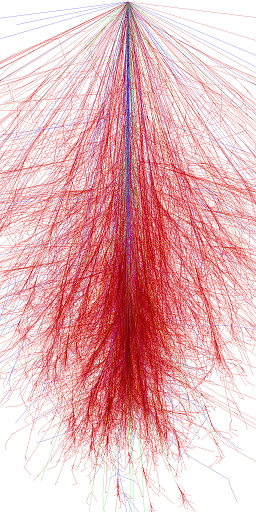
\includegraphics[width=1.5in]{images/ironcascade.png}
    \caption{Cascada atmosférica creada a partir de núcleo de hierro con energía de 1 TeV simulada en CORSIKA. Imagen adoptada de \url{https://www.ikp.kit.edu/corsika/index.php}}
    \label{fig:ironcascade}
\end{figure}

Para la simulación de EAS, un aspecto importante es el modelo de rigidez atmosférica. El programa hace seguimiento, entre otras cosas, a la energía de las partículas de las EAS; si una partícula no tiene una energía lo suficientemente alta como para pasar el umbral establecido por el modelo de rigidez atmosférica, la partícula no podrá continuar su viaje a través de la atmósfera. Además, es bien sabido que el campo magnético terrestre puede afectar el viaje de los rayos cósmicos, alterando su curso y desviándolos de sus trayectorias iniciales. Estos son fenómenos cuyos efectos se pueden tener en cuenta en la simulación de EAS mediante la herramienta MAGNETOCOSMICS de Geant4.

La aplicación de MAGNETOCOSMICS permite calcular la trayectoria de partículas cargadas en la magnetosfera terrestre mediante modelos avanzados del campo geomagnético, y computar los modelos de rigidez atmosférica para el filtrado de partículas. \cite{magnetocosmics} La gran utilidad de esta herramienta hace menester integrarla con las simulaciones de CORSIKA.

Finalmente, Geant4\footnote{\textbf{GE}ometry \textbf{AN}d \textbf{T}racking} es un grupo de herramientas computacionales (\textit{toolkit}) diseñadas para la simulación del paso del paso de partículas a través de materia, simulando procesos de interacciones y decaimientos. Ha sido ampliamento utilizado en las áreas de física de partículas, física nuclear, física de aceleradores, física espacial y estudios médicos. \cite{agostinelli2003geant4}

En este trabajo balancearemos el uso de todas estas herramientas computacionales para simular con rigor la interacción de EAS con la materia de la corteza terrestre.



%---------------------------
%\subsection*{Estado del arte}










%---------------------------
\section*{Plan de trabajo}

\subsection*{Planteamiento y justificación}



\subsection*{Objetivos}

\subsubsection*{General}
\begin{itemize}
    \item Estimar el espectro energético de la radiación, producida por la interacción entre EAS y la corteza terrestre, que ha sido dispersada hacia el exterior de la corteza.
\end{itemize}

\subsubsection*{Específicos}
\begin{enumerate}
    \item Estimar las partículas secundarias producidas en EAS que llegan a interactuar con la corteza terrestre, teniendo en cuenta el efecto de desviación de rayos cósmicos ejercido por el campo geomagnético.
    \item Modelar un volumen de material de corteza terrestre correspondiente a \textit{roca estándar}.
    \item Modelar las interacciones entre las partículas secundarias de las EAS y las partículas del sólido modelo de corteza terrestre.
    \item De los resultados de la interacción entre las EAS y la corteza terrestre, discernir aquellas partículas cuya dirección tiene componente positiva sobre el vector normal a la superficie del suelo de tal forma que son dispersadas de vuelta hacia el exterior de la corteza, y hacer la estimación de su espectro energético.
\end{enumerate}

\subsection*{Metodología}

\begin{enumerate}
    \item Estudiar con rigor la teoría física pertinente para el desarrollo del proyecto; principalmente la teoría concerniente a rayos cósmicos, cascadas atmosféricas extensas, interacción de rayos cósmicos con la materia y detección de rayos cósmicos.
    \item Estudiar el funcionamiento de los \textit{softwares} necesarios, con el fin de tener un buen manejo de estos para llevar a cabo el proyecto. Los programas en cuestión son CORSIKA y MAGNETOCOSMICS para la simulación de EAS, y Geant4 para la simulación de interacciones de partículas de las EAS con la materia de la corteza terrestre.
    \item Realizar un código en Python que facilite, a nivel de usuario, el proceso de simulación de EAS con CORSIKA y MAGNETOCOSMICS. Esto es, crear una interfaz de usuario en Python que permita tener control sobre los parámetros relevantes para la simulación de EAS en CORSIKA, y que integre los resultados de esta a la herramienta MAGNETOCOSMICS, para realizar el proceso de filtrado de partículas por campo geomatnético.
    \item Estudiar el tipo de roca a utilizar, llamada roca estándar, y elaborar un modelo de esta basado en su composición química y demás características relevantes, que pueda ser usado para la simulación con Geant4.
    \item Simular mediante las herramientas disponibles de Geant4 la interacción de las EAS, estimadas en el numeral 3, con el modelo de corteza terrestre (roca estándar), creado en el numeral 4.
    \item De los resultados obtenidos en el numeral 5, discernir aquellas partículas cuya dirección resultante tiene componente positiva sobre el vector normal a la superficie del suelo de tal forma que son dispersadas de vuelta hacia el exterior de la corteza, y hacer la estimación de su espectro energético.
    \item Escribir el libro de tesis con la teoría, desarrollo y resultados del proyecto pertinentes.
\end{enumerate}

\subsection*{Actividades y cronograma}

\subsection*{Presupuesto}




%----------------------------
\printbibliography

\end{document}
